\documentclass[a4paper,12pt]{article} % добавить leqno в [] для нумерации слева
\usepackage[a4paper,top=1.3cm,bottom=2cm,left=1.5cm,right=1.5cm,marginparwidth=0.75cm]{geometry}
%%% Работа с русским языком
\usepackage{cmap}					% поиск в PDF
\usepackage[warn]{mathtext} 		% русские буквы в фомулах
\usepackage[T2A]{fontenc}			% кодировка
\usepackage[utf8]{inputenc}			% кодировка исходного текста
\usepackage[english,russian]{babel}	% локализация и переносы
\usepackage{physics}
\usepackage{multirow}
\usepackage{longtable}

%%% Нормальное размещение таблиц (писать [H] в окружении таблицы)
\usepackage{float}
\restylefloat{table}



\usepackage{graphicx}

\usepackage{wrapfig}
\usepackage{tabularx}

\usepackage{hyperref}
\usepackage[rgb]{xcolor}
\hypersetup{
	colorlinks=true,urlcolor=blue
}

\usepackage{pgfplots}
\pgfplotsset{compat=1.9}

%%% Дополнительная работа с математикой
\usepackage{amsmath,amsfonts,amssymb,amsthm,mathtools} % AMS
\usepackage{icomma} % "Умная" запятая: $0,2$ --- число, $0, 2$ --- перечисление

%% Номера формул
\mathtoolsset{showonlyrefs=true} % Показывать номера только у тех формул, на которые есть \eqref{} в тексте.

%% Шрифты
\usepackage{euscript}	 % Шрифт Евклид
\usepackage{mathrsfs} % Красивый матшрифт

%% Свои команды
\DeclareMathOperator{\sgn}{\mathop{sgn}}

%% Перенос знаков в формулах (по Львовскому)
\newcommand*{\hm}[1]{#1\nobreak\discretionary{}
	{\hbox{$\mathsurround=0pt #1$}}{}}

\date{\today}

\usepackage{gensymb}

\begin{document}

\begin{titlepage}
	\begin{center}
		{\large МОСКОВСКИЙ ФИЗИКО-ТЕХНИЧЕСКИЙ ИНСТИТУТ (НАЦИОНАЛЬНЫЙ ИССЛЕДОВАТЕЛЬСКИЙ УНИВЕРСИТЕТ)}
	\end{center}
	\begin{center}
		{\large Физтех-школа физики и исследований им. Ландау}
	\end{center}
	
	
	\vspace{4.5cm}
	{\huge
		\begin{center}
			{\bf Отчёт о выполнении лабораторной работы 2.1.6}\\
			Эффект Джоуля-Томсона
		\end{center}
	}
	\vspace{2cm}
	\begin{flushright}
		{\LARGE Автор:\\ Сенокосов Арсений Олегович \\
			\vspace{0.2cm}
			Б02-012}
	\end{flushright}
	\vspace{8cm}
	\begin{center}
		Долгопрудный\\
		\today
	\end{center}
\end{titlepage}


\section{Введение}
\textbf{Цель работы:}  \begin{enumerate}
	\item определение изменения температуры углекислого газа при протекании через малопроницаемую перегородку при разных начальных значениях давления и температуры;
	\item вычисление по результатам опытов коэффициентов Ван-дер-Ваальса <<a>> и <<b>>.
\end{enumerate}

\textbf{В работе используются:} трубка с пористой перегородкой; труба Дьюара; термостат; термометры; дифференциальная термопара; микровольтметр; балластный баллон; манометр.
\section{Теоретические сведения}

Эффектом Джоуля–Томсона называется изменение температуры газа, медленно протекающего из области высокого в область низкого давления в условиях хорошей тепловой изоляции. В разреженных газах, которые приближаются по своим свойствам к идеальному газу, при таком течении температура газа не меняется. Эффект Джоуля–Томсона демонстрирует отличие исследуемого газа от идеального.

В работе исследуется изменение температуры углекислого газа при медленном его течении по трубке с пористой перегородкой (риc. \ref{ust}). Трубка 1 хорошо теплоизолирована. Газ из области повышенного давления $ P_1 $ проходит через множество узких и длинных каналов пористой перегородки 2 в область с атмосферным давлением $ P_2 $. Перепад давления $ \Delta P = P_1 - P_2 $ из-за большого сопротивления каналов может быть заметным даже при малой скорости течения газа в трубке. Величина эффекта Джоуля–Томсона определяется по разности температуры газа до и после перегородки.

Рассмотрим стационарный поток газа между произвольными сечениями I и II трубки (до перегородки и после нее). Пусть, для определенности, через трубку прошел 1 моль углекислого газа; $ \mu $ -- его молярная масса. Молярные объемы газа, его давления и отнесенные к молю внутренние энергии газа в сечениях I и II обозначим соответственно $ V_1, P_1, U_1 $ и $ V_2, P_2, U_2 $. Для того чтобы ввести в трубку объем $ V_1 $, над газом нужно совершить работу $ A_1 = P_1V_1 $. Проходя через сечение II, газ сам совершает работу $ A_2 = P_2V_2 $. Так как через боковые стенки не происходит ни обмена теплом, ни передачи механической энергии, то

\begin{equation}\label{1}
A_1-A_2=\left(U_2+\frac{\mu v_2^2}{2}\right) - \left(U_1 + \frac{\mu v_1^2}{2}\right).
\end{equation}

В уравнении \eqref{1} учтено изменение как внутренней (первые члены в скобках), так и кинетической (вторые члены в скобках) энергии газа. Подставляя в \eqref{1} написанные выражения для $ A_1 $ и $ A_2 $ и перегруппировывая члены, найдем

\begin{equation}\label{2}
H_1-H_2=\left(U_1+P_1V_1\right) - \left(U_2 + P_2V_2\right) = \frac{1}{2} \mu \left(v^2_2-v^2_1\right).
\end{equation}

Сделаем несколько замечаний. Прежде всего отметим, что в процессе Джоуля–Томсона газ испытывает в пористой перегородке существенное трение, приводящее к ее нагреву. Потери энергии на нагрев трубки в начале процесса могут быть очень существенными и сильно искажают ход явления. После того как температура трубки установится и газ станет уносить с собой все выделенное им в пробке тепло, формула \eqref{1} становится точной, если, конечно, теплоизоляция трубки достаточно хороша и не происходит утечек тепла наружу через ее стенки.

Второе замечание связано с правой частью \eqref{2}. Процесс Джоуля–Томсона в чистом виде осуществляется лишь в том случае, если правой частью можно пренебречь, т. е. если макроскопическая скорость газа с обеих сторон трубки достаточно мала. У нас сейчас нет критерия, который позволил бы установить, когда это можно сделать. В силу сохранения энтропии в случае реального газа получаем:

\begin{equation}\label{3}
\mu_\text{Д--Т} = \frac{\Delta T}{\Delta P} \approx \frac{(2a/RT) - b}{C_P}.
\end{equation}

Из формулы \eqref{3} видно, что эффект Джоуля–Томсона для не очень плотного газа зависит от соотношения величин $ a $ и $ b $, которые оказывают противоположное влияние на знак эффекта. Если силы взаимодействия между молекулами велики, так что превалирует <<поправка на давление>>, то основную роль играет член, содержащий $ a $, и 

\[ \frac{\Delta T}{\Delta P} > 0, \]
т. е. газ при расширении охлаждается ($ \Delta T < 0 $, так как всегда $ \Delta P < 0 $). В обратном случае (малые $ a $)

\[ \frac{\Delta T}{\Delta P} < 0, \]
т. е. газ нагревается ($ \Delta T > 0 $, так как по-прежнему $ \Delta P < 0 $).

Этот результат нетрудно понять из энергетических соображений. Как мы уже знаем, у идеального газа эффект Джоуля–Томсона отсутствует. Идеальный газ отличается от реального тем, что в нем можно пренебречь потенциальной энергией взаимодействия молекул. Наличие этой энергии приводит к охлаждению или нагреванию реальных газов при расширении. При больших a велика энергия притяжения молекул. Это означает, что потенциальная энергия молекул при их сближении уменьшается, а при удалении -- при расширении газа -- возрастает. Возрастание потенциальной энергии молекул происходит за счет их кинетической энергии -- температура газа при расширении падает. Аналогичные рассуждения позволяют понять, почему расширяющийся газ нагревается при больших значениях $ b $.

Как следует из формулы \eqref{3}, при температуре \[ T_i = \frac{2a}{Rb} \] коэффициент $ \mu_\text{Д--Т} $ обращается в нуль. По формулам связи параметров газа Ван-дер-Ваальса с критическими параметрами получаем: 

\begin{equation}\label{4}
T_\text{инв} = \frac{27}{4} T_\text{кр}.
\end{equation}

При температуре $ T_\text{инв} $ эффект Джоуля–Томсона меняет знак: ниже температуры инверсии эффект положителен ($ \mu_\text{Д--Т} > 0 $, газ охлаждается), выше $ T_\text{инв} $ эффект отрицателен ($ \mu_\text{Д--Т} < 0 $, газ нагревается).

Вернемся к влиянию правой части уравнения \eqref{2} на изменение температуры расширяющегося газа. Для этого сравним изменение температуры, происходящее вследствие эффекта Джоуля–Томсона, с изменением температуры, возникающим из-за изменения кинетической энергии газа. Увеличение кинетической энергии газа вызывает заметное и приблизительно одинаковое понижение его температуры как у реальных, так и у идеальных газов. Поэтому при оценках нет смысла пользоваться сложными формулами для газа Ван-дер-Ваальса.

Заменяя в формуле \eqref{2} $ U $ через $ C_VT $ и $ PV $ через $ RT $, найдем

\[ \left(R+C_V\right)\left(T_1-T_2\right)=\mu\left(v_2^2-v_1^2\right)/2 \]
или
\[ \Delta T = \frac{\mu}{2C_P}\left(v_2^2-v_1^2\right). \]

В условиях нашего опыта расход газа $ Q  $ на выходе из пористой перегородки не превышает $ 10 $ см$ ^3 $/с, а диаметр трубки равен 3 мм. Поэтому

\[ v_2<=\frac{4Q}{\pi d^2} = \frac{4\cdot\text{см}^3/\text{с}}{3,14\cdot(0,3)^2\text{ см}^2} \approx 140 \text{ см}/\text{с}. \]

Скорость $ v_1 $ газа у входа в пробку относится к скорости $ v_2 $ у выхода из нее как давление $ P_2 $ относится к $ P_1 $. В нашей установке $ P_1 = 4 $ атм, a $ P_2 = 1 $ атм, поэтому

\[ v_1=\frac{P_2}{P_1}v_2 = 35 \text{ см}/\text{с}. \]

Для углекислого газа $ \mu = 44 $ г/моль, $ C_P = 40 $ Дж/(моль·К); имеем

\[ \Delta T = \frac{\mu}{2C_P}\left(v_2^2-v_1^2\right) \approx 7\cdot10^{-4} \text{ K}. \]

Это изменение температуры ничтожно мало по сравнению с измеряемым эффектом (несколько градусов).

В данной лабораторной работе исследуется коэффициент дифференциального эффекта Джоуля–Томсона для углекислого газа. По экспериментальным результатам оценивается коэффициент теплового расширения, постоянные в уравнении Ван-дер-Ваальса и температура инверсии углекислого газа. Начальная температура газа $ T_1 $ задается термостатом. Измерения проводятся при трех температурах: комнатной, 30 $ ^\circ $C и 50 $ ^\circ $C.

\section{Экспериментальная установка}

\begin{figure}[H]
	\begin{center}
		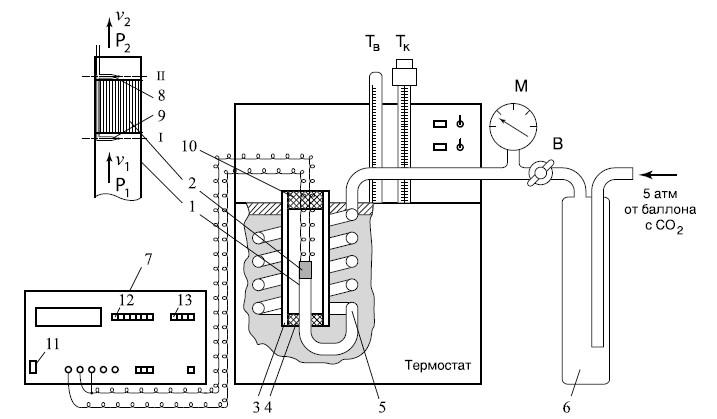
\includegraphics[width=18cm]{ust.jpg}
	\end{center}
	\caption{\textit{Схема установки}}
	\label{ust}
\end{figure}

Схема установки для исследования эффекта Джоуля–Томсона в углекислом газе представлена на рисунке \ref{ust}. Основным элементом установки является трубка 1 с пористой перегородкой 2, через которую пропускается исследуемый газ. Трубка имеет длину 80 мм и сделана из нержавеющей стали, обладающей, как известно, малой теплопроводностью. Диаметр трубки $ d = 3 $~мм, толщина стенок 0,2 мм. Пористая перегородка расположена в конце трубки и представляет собой стеклянную пористую пробку со множеством узких и длинных каналов. Пористость и толщина пробки ($ l = 5 $ мм) подобраны так, чтобы обеспечить оптимальный поток газа при перепаде давлений $ \Delta P = 4 $ атм (расход газа составляет около $ 10 $ см$ ^3 $/с); при этом в результате эффекта Джоуля–Томсона создается достаточная разность температур.

Углекислый газ под повышенным давлением поступает в трубку через змеевик 5 из балластного баллона 6. Медный змеевик омывается водой и нагревает медленно протекающий через него газ до температуры воды в термостате. Температура воды измеряется термометром $ T_\text{в} $, помещенным в термостате. Требуемая температура воды устанавливается и поддерживается во время эксперимента при помощи контактного термометра $ T_\text{к} $.

Давление газа в трубке измеряется манометром М и регулируется вентилем В (при открывании вентиля В, т. е. при повороте ручки против часовой стрелки, давление $ P_1 $ повышается). Манометр М измеряет разность между давлением внутри трубки и наружным (атмосферным) давлением. Так как углекислый газ после пористой перегородки выходит в область с атмосферным давлением $ P_2 $, то этот манометр непосредственно измеряет перепад давления на входе и на выходе трубки $ \Delta P = P_1 - P_2 $.

Разность температур газа до перегородки и после нее измеряется дифференциальной термопарой медь -- константан. Константановая проволока диаметром 0,1 мм соединяет спаи 8 и 9, а медные проволоки (того же диаметра) подсоединены к цифровому вольтметру 7. Отвод тепла через проволоку столь малого сечения пренебрежимо мал. Для уменьшения теплоотвода трубка с пористой перегородкой помещена в трубу Дьюара 3, стенки которой посеребрены, для уменьшения теплоотдачи, связанной с излучением. Для уменьшения теплоотдачи за счет конвекции один конец трубы Дьюара уплотнен кольцом 4, а другой закрыт пробкой 10 из пенопласта. Такая пробка практически не создает перепада давлений между внутренней полостью трубы и атмосферой.

\section{Ход работы}

\subsection{Определение коэффициента Джоуля-Томсона}

Проведём измерение зависимости $ \Delta T $ от $ \Delta P $ для разных значений температур. Полученные значения заносим в таблицы \ref{tab:20C}, \ref{tab:30C} и \ref{tab:50C}. При записи полученных данных также учитываем, что чувствительность термопары медь -- константан зависит от температуры. При вычислении будем использовать следующую формулу: \[ \Delta T = \frac{U}{\alpha}, \] где \[ \alpha_{20^\circ C} = 40,2 \text{ мкВ}/^\circ C, \quad \alpha_{30^\circ C} = 41,1 \text{ мкВ}/^\circ C, \quad \alpha_{50^\circ C} = 42,9 \text{ мкВ}/^\circ C . \]


\begin{table}[H]
	\centering
	\begin{tabular}{|c|c|c|c|c|c|}
		\hline
		\multicolumn{6}{|c|}{$ T = 20 \text{ } ^\circ C $} \\ \hline
		$ \Delta P $, атм & $ \sigma_p $, атм & $ U $, мВ & $ \sigma_U $, мВ & $ \Delta T $, K & $ \sigma_{\Delta T} $, K \\ \hline
		4,00 & 0,05 & 0,156 & 0,001 & 4,05 & 0,02 \\ \hline
		3,50 & 0,05 & 0,132 & 0,001 & 3,46 & 0,02 \\ \hline
		3,00 & 0,05 & 0,108 & 0,001 & 2,86 & 0,02 \\ \hline
		2,50 & 0,05 & 0,088 & 0,001 & 2,36 & 0,02 \\ \hline
		2,00 & 0,05 & 0,066 & 0,001 & 1,82 & 0,02 \\ \hline
		1,50 & 0,05 & 0,045 & 0,001 & 1,29 & 0,02 \\ \hline
		1,00 & 0,05 & 0,026 & 0,001 & 0,82 & 0,02 \\ \hline
		0,50 & 0,05 & 0,008 & 0,001 & 0,37 & 0,02 \\ \hline
	\end{tabular}
	\caption{Экспериментальные данные для 20 $^\circ$C}
	\label{tab:20C}
\end{table}

\begin{table}[H]
	\centering
	\begin{tabular}{|c|c|c|c|c|c|}
		\hline
		\multicolumn{6}{|c|}{$ T = 30 \text{ } ^\circ C $} \\ \hline
		$ \Delta P $, атм & $ \sigma_p $, атм & $ U $, мВ & $ \sigma_U $, мВ & $ \Delta T $, K & $ \sigma_{\Delta T} $, K \\ \hline
		4,00 & 0,05 & 0,144 & 0,001 & 3,67 & 0,02 \\ \hline
		3,50 & 0,05 & 0,123 & 0,001 & 3,16 & 0,02 \\ \hline
		3,00 & 0,05 & 0,100 & 0,001 & 2,60 & 0,02 \\ \hline
		2,50 & 0,05 & 0,080 & 0,001 & 2,12 & 0,02 \\ \hline
		2,00 & 0,05 & 0,060 & 0,001 & 1,63 & 0,02 \\ \hline
		1,50 & 0,05 & 0,040 & 0,001 & 1,14 & 0,02 \\ \hline
		1,00 & 0,05 & 0,020 & 0,001 & 0,66 & 0,02 \\ \hline
		0,50 & 0,05 & 0,008 & 0,001 & 0,36 & 0,02 \\ \hline
	\end{tabular}
	\caption{Экспериментальные данные для 30 $^\circ$C}
	\label{tab:30C}
\end{table}

\begin{table}[H]
	\centering
	\begin{tabular}{|c|c|c|c|c|c|}
		\hline
		\multicolumn{6}{|c|}{$ T = 50 \text{ } ^\circ C $} \\ \hline
		$ \Delta P $, атм & $ \sigma_p $, атм & $ U $, мВ & $ \sigma_U $, мВ & $ \Delta T $, K & $ \sigma_{\Delta T} $, K \\ \hline
		4,00 & 0,05 & 0,127 & 0,001 & 3,12 & 0,02 \\ \hline
		3,50 & 0,05 & 0,107 & 0,001 & 2,66 & 0,02 \\ \hline
		3,00 & 0,05 & 0,088 & 0,001 & 2,21 & 0,02 \\ \hline
		2,50 & 0,05 & 0,069 & 0,001 & 1,77 & 0,02 \\ \hline
		2,00 & 0,05 & 0,051 & 0,001 & 1,35 & 0,02 \\ \hline
		1,50 & 0,05 & 0,034 & 0,001 & 0,96 & 0,02 \\ \hline
		1,00 & 0,05 & 0,019 & 0,001 & 0,61 & 0,02 \\ \hline
		0,50 & 0,05 & 0,008 & 0,001 & 0,35 & 0,02 \\ \hline
	\end{tabular}
	\caption{Экспериментальные данные для 50 $^\circ$C}
	\label{tab:50C}
\end{table}

Также необходимо учесть, что при $ \Delta P = 0$ показания вольтметра составляли $ U(0) =~-0,007 $~мкВ. Поэтому для корректной обработки данных сделаем необходимую поправку, вычитая из полученных показаний $ U(0) $.

Кроме того, при вычислении $ \Delta T $ погрешность этого вычисления определяем по формуле: \[ \sigma_{\Delta T} = \Delta T \frac{\sigma_U}{U}. \]

По имеющимся данным проведём аппроксимацию зависимости $ \Delta T $ от $ \Delta P $, чтобы определить коэффициент Джоуля-Томсона. На рисунке \ref{ris} изображены графики зависимостей.



Вычислим $ \mu_\text{Д--Т} = \frac{dT}{dP} $, используя метод наименьших квадратов:

\[ \mu_\text{Д--Т} = \frac{\langle \Delta P \Delta T \rangle - \langle \Delta P \rangle \langle \Delta T \rangle}{\langle \Delta P \rangle - \langle \Delta P \rangle ^2}.\]

Случайную погрешность определения этого коэффициента вычислим по следующей~формуле:

\[ \sigma^\text{случ}_{\mu_\text{Д--Т}} = \sqrt{\frac{1}{N-2} \left(\frac{\left\langle\left(\Delta T - \langle \Delta T\right\rangle\right)^2 \rangle}{\left\langle\left(\Delta P - \langle \Delta P\right\rangle\right)^2 \rangle}\right)-\mu_\text{Д--Т}^2},\] где  $ N $  -- колличество измерений.



Систематические погрешности оценим по следующим формуле:

\[ \sigma^\text{сист}_{\mu_\text{Д--Т}} = {\mu_\text{Д--Т}}\sqrt{\varepsilon^2_{\Delta P}+\varepsilon^2_{\Delta T}}.\]

\begin{figure}[H]
	\caption{Графики зависимости $ \Delta T $ от $ \Delta P $}\label{ris}
	\begin{center}
		\begin{tikzpicture}
		\begin{axis}[
		xlabel={$ \Delta P $, атм},
		ylabel={$\Delta T$, \textdegree K},
		legend pos=north west,
		xmajorgrids=true,
		ymajorgrids=true,
		grid style=dashed,
		width = 520,
		height = 350,
		%xmin = 300,
		%xmax = 335,
		%ymin =40,
		%ymax =135,
		]
		\legend{ 
			,,,
			$ T=20^\circ C $,
			$ T=30^\circ C $,
			$ T=50^\circ C $
		};
		\addplot+ [blue, only marks, mark size = 4pt,
		error bars/.cd,
		x dir=both, x explicit,
		y dir=both, y explicit, 
		] table [x = P, y = T, x error = dP, y error = dT,] {
			P	dP	T	dT                  
			4.00	0.05	4.054726368	0.024875622
			3.50	0.05	3.457711443	0.024875622
			3.00	0.05	2.860696517	0.024875622
			2.50	0.05	2.36318408	0.024875622
			2.00	0.05	1.815920398	0.024875622
			1.50	0.05	1.293532338	0.024875622
			1.00	0.05	0.820895522	0.024875622
			0.50	0.05	0.373134328	0.024875622
			
		};
		\addplot+ [blue, only marks, mark size = 4pt,
		error bars/.cd,
		x dir=both, x explicit,
		y dir=both, y explicit, 
		] table [x = P, y = T, x error = dP, y error = dT,] {
			P	dP	T	dT                  
			4.00	0.05	3.673965937	0.0243309
			3.50	0.05	3.163017032	0.0243309
			3.00	0.05	2.603406326	0.0243309
			2.50	0.05	2.116788321	0.0243309
			2.00	0.05	1.630170316	0.0243309
			1.50	0.05	1.143552311	0.0243309
			1.00	0.05	0.656934307	0.0243309
			0.50	0.05	0.364963504	0.0243309
			
		};
		\addplot+ [blue, only marks, mark size = 4pt,
		error bars/.cd,
		x dir=both, x explicit,
		y dir=both, y explicit, 
		] table [x = P, y = T, x error = dP, y error = dT,] {
			P	dP	T	dT                  
			4.00	0.05	3.12354	0.023310023
			3.50	0.05	2.65734	0.023310023
			3.00	0.05	2.21445	0.023310023
			2.50	0.05	1.77156	0.023310023
			2.00	0.05	1.35198	0.023310023
			1.50	0.05	0.95571	0.023310023
			1.00	0.05	0.60606	0.023310023
			0.50	0.05	0.34965	0.023310023
		};
		\addplot [red, domain=0.5:4, line width =3.2pt] {-0.238095238+1.052475717*x};
		\addplot [blue, domain=0.5:4, line width =3.2pt] {-0.253736531+0.965705017*x};
		\addplot [green, domain=0.5:4, line width =3.2pt] {-0.185647686+0.806415806*x};
		\end{axis}
		\end{tikzpicture}
	\end{center}
	
\end{figure}

Таким образом, полная погрешность измерения определяется следующим соотношением:

\[ \sigma_{\mu_\text{Д--Т}} = \sqrt{(\sigma_{\mu_\text{Д--Т}}^\text{сист})^2 + (\sigma_{\mu_\text{Д--Т}}^\text{случ})^2}.\]

Результаты вычислений заносим в таблицу \ref{tab:my-table}.
\label{koef}
\begin{table}[H]
	\centering
	\begin{tabular}{|c|c|c|c|}
		\hline
		$ T $, $ ^\circ C $ & $ \mu_\text{Д--Т} $, К/атм & $ \sigma_{\mu_\text{Д--Т}} $, К/атм & $ \varepsilon $, $ \% $ \\ \hline
		20 & 1,05 & 0,02 & 2,3 \\ \hline
		30 & 0,97 & 0,03 & 2,8 \\ \hline
		50 & 0,81 & 0,03 & 3,4 \\ \hline
	\end{tabular}
	\caption{Результаты измерений $ \mu_\text{Д--Т} $}
	\label{tab:my-table}
\end{table}

\subsection{Вычисление параметров газа Ван-дер-Ваальса}

Вычислим параметры газа Ван-дер-Ваальса, используя коэффициенты $ \mu_\text{Д--Т} $, полученные в \ref{koef}, для разных пар температур.

Пользуясь формулой \eqref{3}, получим 

\[ \left\{ \begin{aligned}
	 a &= \frac{\left(\mu_1 - \mu_2\right)C_PRT_1T_2}{2\left(T_2-T_1\right)}, \\
	b &= \frac{C_P(\mu_2T_2-\mu_1T_1)}{T_1-T_2}. \end{aligned} \right. \]

Погрешности этих вычислений можно оценить используя следующие формулы:~\[ \sigma_a = a\sqrt{\varepsilon^2_{\mu_1-\mu_2}+\varepsilon^2_{T_1}+\varepsilon^2_{T_2}+\varepsilon^2_{T_2-T_1}}, \] \[ \sigma_b=b\sqrt{\varepsilon^2_{\mu_2T_2-\mu_1T_1}+\varepsilon^2_{T_1-T_2}}, \] где \[ \sigma_{x\pm y} =\sqrt{\sigma^2_x+\sigma^2_y}. \]

Для температур 20$ ^\circ $C и 30$ ^\circ $C, а также для 30$ ^\circ $C и 50$ ^\circ $C, вычисляем параметры <<a>> и <<b>> газа Ван-дер-Ваальса. Результаты вычислений заносим в таблицу \ref{tab:a-b}.

\begin{table}[H]
	\centering
	\begin{tabular}{|c|c|c|c|c|c|c|}
		\hline
		$ T $, $ ^\circ C $ & $ a $, $\displaystyle \frac{\text{Па}\cdot\text{м}^6}{\text{моль}^2} $ &$ \sigma_a $, $\displaystyle \frac{\text{Па}\cdot\text{м}^6}{\text{моль}^2} $ & $ \varepsilon_a $, \% & $ b\cdot10^{-4} $, $ \displaystyle\frac{\text{м}^3}{\text{моль}} $ & $ \sigma_b \cdot 10^{-4} $, $\displaystyle \frac{\text{м}^3}{\text{моль}} $ & $ \varepsilon_b $, \% \\ \hline
		30 -- 20 & 1,30 & 0,55 & 42,1 & 6,38 & 4,42 & 69,2 \\ \hline
		50 -- 30 & 1,31 & 0,32 & 24,4 & 6,50 & 2,46 & 37,9 \\ \hline
	\end{tabular}
	\caption{Результаты измерения параметров газа Ван-дер-Ваальса}
	\label{tab:a-b}
\end{table}

Сверим полученные результаты с табличными. Согласно справочнику для углекислого газа \[ a = 0,36 \text{ } \frac{\text{Па}\cdot\text{м}^6}{\text{моль}^2}, \] \[ b = 0,42\cdot 10^{-4} \text{ }\frac{\text{м}^3}{\text{моль}}. \]

Полученные данные значительно отличаются от табличных. Про причины такого различия сказано в выводе.

\subsection{Вычисление температуры инверсии}

Используя формулу \eqref{4}, по полученным параметрам газа Ван-дер-Ваальса вычислим $ T_\text{инв} $. Также оценим погрешность по следующей формуле:

\[ \sigma_{T_\text{инв}} = T_\text{инв}\sqrt{\varepsilon^2_a+\varepsilon_b^2}. \]

Результаты вычислений занесём в таблицу \ref{tab:temp}.

\begin{table}[H]
	\centering
	\begin{tabular}{|c|c|c|c|}
		\hline
		$ T $, $ ^\circ C $ & $ T_\text{инв} $, $ ^\circ $К & $ \sigma_{T_\text{инв}} $, $ ^\circ $К & $ \varepsilon $, \% \\ \hline
		30-20 & 489 & 396 & 81 \\ \hline
		50-30 & 485 & 219 & 45 \\ \hline
	\end{tabular}
	\caption{Результаты вычисления температуры инверсии}
	\label{tab:temp}
\end{table}

Для углекислого газа, согласно справочнику  \[ T_\text{инв} = 2053 \text{ K}.\]

Полученные результаты снова сильно отличаются от табличных.

\section{Обсуждение результатов и выводы}

В ходе выполнения работы мы:

\begin{itemize}
	\item экспериментальным методом измерили коэффициенты газа Ван-дер-Ваальса <<a>> и <<b>>;
	\item вычислили $ T_\text{инв} $ для углекислого газа.
\end{itemize}

В ходе работы мы получили значения, очень сильно отличающиеся от табличных. Погрешность вычисления параметров газа Ван-дер-Ваальса составила десятки процентов. Такая большая ошибка может говорить нам о неприменимости уравнения Ван-дер-Ваальса в условия лабораторной работы. Действительно, это уравнение используется лишь для качественного описания процессов, происходящих с реальными газами. Количественный подход к этому уравнению неприменим.

Также для увеличения точности измерений можно использовать более точные методы измерения температуры. Повысить точность необходимо как у термостата, так и у вольтметра, т.к. температура на них колебалась на протяжении эксперимента, несмотря на то, что условия оставались неизменными.

\section{Контрольные вопросы}

\begin{enumerate}
	\item Реальные газы отличаются от своей модели -- идеальных газов -- тем, что их молекулы имеют конечные размеры и между ними действуют силы притяжения (при
	значительных расстояниях между молекулами) и отталкивания (при сближении молекул друг с другом).
	\item Для потенциальной энергии двух молекул можно записать потенциал Леннарда-Джонса: \[ U(r)=4\varepsilon\left[\left(\frac{\sigma}{r}\right)^{12}-\left(\frac{\sigma}{r}\right)^6\right]. \] Ниже изображён характерный вид потенциала Леннарда-Джонса:
	
	\begin{center}
		\begin{tikzpicture}
		\begin{axis}[
		axis lines=middle,
		xlabel={$\displaystyle \frac{\sigma}{r} $},
		ylabel={$\displaystyle \frac{U}{4\varepsilon} $},
		legend pos=north west,
		xmajorgrids=true,
		ymajorgrids=true,
		grid style=dashed,
		width = 500,
		height = 360,
		ymin =-0.27,
		ymax =0.5,
		xmin =0.93,
		xmax =1.7,
		]
		\addplot [red, domain=0.95:1.7, line width =1.5pt, samples = 100] {(1/x^12)-(1/x^6)};
		\end{axis}
		\end{tikzpicture}
	\end{center}
	Чтобы получить силу, продифференцируем уравнение для потенциальной энергии: \[ 
	F(r)=-\frac{\partial}{\partial r}\left(4\varepsilon\left[\left(\frac{\sigma}{r}\right)^{12}-\left(\frac{\sigma}{r}\right)^6\right]\right)=-24\varepsilon\left(\frac{\sigma^6}{r^7}-2\frac{\sigma^{12}}{r^{13}}\right).
	 \]
	 Ниже на графики изображён характерный вид зависимости силы от расстояния между молекулами:
	 \begin{center}
	 	\begin{tikzpicture}
	 	\begin{axis}[
	 	axis lines=middle,
	 	xlabel={$\displaystyle \frac{\sigma}{r} $},
	 	ylabel={$\displaystyle \frac{F\sigma}{24\varepsilon} $},
	 	legend pos=north west,
	 	xmajorgrids=true,
	 	ymajorgrids=true,
	 	grid style=dashed,
	 	width = 500,
	 	height = 360,
	 	ymin =-0.25,
	 	ymax =0.5,
	 	xmin =0.93,
	 	xmax =1.7,
	 	]
	 	\addplot [red, domain=0.95:1.7, line width =1.5pt, samples = 100] {(1/x^13)-(1/x^7)};
	 	\end{axis}
	 	\end{tikzpicture}
	 \end{center}
 По этим графикам можно объяснить причины эффекта Джоуля–Томсона. Заметим,
 что при увеличении расстояния между двумя молекулами, они совершают работу,
 против силы взаимодействия, а также их потенциальная энергия взаимодействия
 изменяется. Так как система замкнута, то происходит изменение внутренних энергий
 молекул, так что газ охлаждается.
 \item Критическая температура определяется как температура, при которой исчезают различия в физических свойствах между жидкостью и паром, находящимися в равновесии.
 
 Температура инверсии -- температура, при которой изменение температуры в дифференциальном эффекте отсутствует.
 \item При $ a \neq 0, b = 0 $ велика энергия притяжения молекул. Это означает, что потенциальная энергия молекул при их сближении уменьшается, а при удалении -- при  расширении газа -- возрастает. Возрастание потенциальной энергии молекул происходит за счёт их кинетической энергии -- температура газа при расширении падает.
 Аналогичные рассуждения позволяют понять, почему расширяющийся газ нагревается при $ a = 0, b \neq 0 $.

\end{enumerate} 

















\end{document}